\documentclass[aspectratio=169,10pt]{beamer}

\usetheme{default}
\usefonttheme{professionalfonts}
\setbeamertemplate{navigation symbols}{}
\setbeamersize{text margin left=0.75cm,text margin right=0.75cm}

\usepackage[T1]{fontenc}
\usepackage{amsmath,amssymb}
\usepackage{array}
\usepackage{booktabs}
\usepackage{colortbl}
\usepackage{graphicx}
\usepackage{tikz}
\usepackage{xspace}
\usetikzlibrary{arrows.meta,calc,positioning}

% Supports compilation from either pmds/latex or the repository root.
\graphicspath{{../results/plots/}{pmds/results/plots/}}

\definecolor{Ink}{HTML}{17212B}
\definecolor{Muted}{HTML}{66717D}
\definecolor{Paper}{HTML}{F7F9FA}
\definecolor{Line}{HTML}{D9E0E5}
\definecolor{Teal}{HTML}{087E8B}
\definecolor{TealLight}{HTML}{DCEFF0}
\definecolor{Coral}{HTML}{D95D39}
\definecolor{CoralLight}{HTML}{F8E4DE}
\definecolor{Gold}{HTML}{C58B13}
\definecolor{GoldLight}{HTML}{F6ECD2}
\definecolor{Green}{HTML}{2E7D5B}
\definecolor{GreenLight}{HTML}{DDEEE6}
\definecolor{Red}{HTML}{B53A3A}
\definecolor{RedLight}{HTML}{F5DEDE}

\setbeamercolor{normal text}{fg=Ink,bg=white}
\setbeamercolor{frametitle}{fg=Ink}
\setbeamercolor{structure}{fg=Teal}
\setbeamercolor{itemize item}{fg=Teal}
\setbeamercolor{itemize subitem}{fg=Teal}
\setbeamerfont{frametitle}{size=\Large,series=\bfseries}
\setbeamerfont{title}{series=\bfseries}
\setbeamerfont{footline}{size=\scriptsize}

\setbeamertemplate{frametitle}{
  \vspace{0.28cm}
  \insertframetitle\par
  \vspace{0.10cm}
  {\color{Teal}\rule{\linewidth}{0.7pt}}
}
\setbeamertemplate{footline}{
  \leavevmode
  \hbox to \paperwidth{%
    \hspace{0.75cm}%
    {\usebeamerfont{footline}\color{Muted}Amirhossein Bagheri}%
    \hfill
    {\usebeamerfont{footline}\color{Muted}PMDS Forecasting Project
      \quad \insertframenumber/\inserttotalframenumber}%
    \hspace{0.42cm}%
  }
  \vspace{0.22cm}
}
\setbeamertemplate{itemize item}{\raise0.2ex\hbox{\small$\blacktriangleright$}}
\setbeamertemplate{itemize subitem}{\raise0.2ex\hbox{\scriptsize$\bullet$}}

\newcommand{\system}{\textsc{PMDS Forecasting Project}\xspace}
\newcommand{\key}[1]{{\color{Teal}\textbf{#1}}}
\newcommand{\bad}[1]{{\color{Coral}\textbf{#1}}}
\newcommand{\good}[1]{{\color{Green}\textbf{#1}}}
\newcommand{\scorebox}[2]{%
  \colorbox{#1}{\makebox[15mm][c]{\strut\textbf{#2}}}%
}
\newcommand{\tagbox}[2]{%
  \tikz[baseline=(tag.base)]{
    \node[fill=#1,rounded corners=1.5pt,inner xsep=6pt,inner ysep=3pt]
      (tag) {\strut #2};
  }%
}
\newcolumntype{L}[1]{>{\raggedright\arraybackslash}p{#1}}
\newcolumntype{C}[1]{>{\centering\arraybackslash}p{#1}}

\title{\system: Foundation Model vs. Classical Methods}
\author{Amirhossein Bagheri}
\institute{Politecnico di Milano \qquad Supervisor: Tommaso Bianchi}
\date{}

\begin{document}

% ------------------------------------------------------------
\begin{frame}[plain]
  \vspace{0.45cm}
  {\color{Teal}\rule{1.25cm}{3pt}}

  \vspace{0.45cm}
  {\fontsize{25}{30}\selectfont\bfseries
    Chronos T5 Tiny vs.\\[2pt]
    Classical Forecasting Methods\par}

  \vspace{0.38cm}
  {\Large\color{Muted}
    An applied foundation-model comparison across six datasets,\\
    nine models, and five metrics\par}

  \vspace{0.42cm}
  \tagbox{TealLight}{\small\textbf{Foundation}: Chronos T5 Tiny}
  \hspace{0.18cm}
  \tagbox{GoldLight}{\small\textbf{Classical}: seven methods}
  \hspace{0.18cm}
  \tagbox{GreenLight}{\small\textbf{Neural reference}: DeepAR}

  \vfill
  {\small\color{Muted}Prepared by}\par
  \vspace{0.08cm}
  {\large\bfseries Amirhossein Bagheri}

  \vspace{0.18cm}
  {\small\color{Muted}
    Politecnico di Milano \qquad Supervisor: Tommaso Bianchi}
\end{frame}


% ------------------------------------------------------------
\begin{frame}{What the project compares}
  \vspace{0.30cm}

  \begin{center}
    \begin{minipage}{0.88\linewidth}
      \Large\raggedright
      Evaluate whether Chronos T5 Tiny, a pretrained
      \key{foundation time-series model}, can match or outperform
      \key{classical forecasting methods} under one common pipeline.
      DeepAR remains a separate neural reference.
    \end{minipage}
  \end{center}

  \vspace{0.62cm}

  \begin{columns}[T,totalwidth=0.92\linewidth]
    \begin{column}{0.28\linewidth}
      \tagbox{TealLight}{\small\textbf{Accuracy comparison}}

      \vspace{0.35cm}
      Which model minimizes median-forecast error?
    \end{column}
    \begin{column}{0.28\linewidth}
      \tagbox{GreenLight}{\small\textbf{Uncertainty comparison}}

      \vspace{0.35cm}
      Which model produces the best quantile forecasts?
    \end{column}
    \begin{column}{0.28\linewidth}
      \tagbox{GoldLight}{\small\textbf{Practical tradeoffs}}

      \vspace{0.35cm}
      Is the comparison valid, and what does each method cost to run?
    \end{column}
  \end{columns}

  \vspace{0.58cm}
\end{frame}

% ------------------------------------------------------------
\begin{frame}{Historical snapshot: six datasets and nine models}
  \vspace{0.20cm}

  \begin{center}
    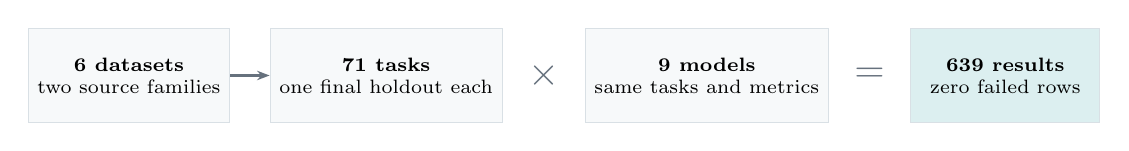
\begin{tikzpicture}[
      node distance=2.5mm,
      factor/.style={draw=Line,fill=Paper,align=center,minimum width=24mm,
        minimum height=12mm,font=\scriptsize},
      arrow/.style={-{Stealth[length=4.5pt]},thick,color=Muted},
      times/.style={font=\Large\bfseries,color=Muted}
    ]
      \node[factor] (datasets) {\textbf{6 datasets}\\two source families};
      \node[factor,right=5mm of datasets] (tasks) {\textbf{71 tasks}\\one final holdout each};
      \node[times,right=2mm of tasks] (x1) {$\times$};
      \node[factor,right=2mm of x1] (models) {\textbf{9 models}\\same tasks and metrics};
      \node[times,right=2mm of models] (eq) {$=$};
      \node[factor,fill=TealLight,right=2mm of eq] (results) {\textbf{639 results}\\zero failed rows};
      \draw[arrow] (datasets) -- (tasks);
    \end{tikzpicture}
  \end{center}

  \vspace{0.45cm}

  \begin{columns}[T,totalwidth=0.96\linewidth]
    \begin{column}{0.50\linewidth}
      \scriptsize
      \renewcommand{\arraystretch}{1.18}
      \setlength{\tabcolsep}{2pt}
      \begin{tabular}{L{0.42\linewidth} C{0.15\linewidth} C{0.15\linewidth} C{0.17\linewidth}}
        \toprule
        \textbf{Dataset} & \textbf{Tasks} & \textbf{Horizon} & \textbf{Lag} \\
        \midrule
        M1 yearly & 20 & 6 & 1 \\
        M4 hourly & 20 & 48 & 24 \\
        Weather & 20 & 30 & 7 \\
        National illness & 1 & 24 & 52 \\
        Traffic & 5 & 24 & 24 \\
        PSM & 5 & 24 & 24 \\
        \bottomrule
      \end{tabular}
    \end{column}

    \begin{column}{0.42\linewidth}
      \small
      \textbf{Model families}
      \begin{itemize}
        \item \key{Foundation model}: Chronos T5 Tiny
        \item \key{Classical methods}: seasonal naive, AR, MA,
          ARMA, ARIMA, AutoARIMA, Prophet
        \item \key{Additional neural reference}: DeepAR
      \end{itemize}

      \vspace{0.22cm}
      {\color{Muted}\scriptsize Historical single-origin run. The repaired full rerun is pending.}
    \end{column}
  \end{columns}
\end{frame}

% ------------------------------------------------------------
\begin{frame}{Read the metric before reading the ranking}
  \vspace{0.08cm}

  \begin{columns}[T,totalwidth=0.95\linewidth]
    \begin{column}{0.47\linewidth}
      \scriptsize
      \tagbox{TealLight}{\textbf{Point forecast metrics}}

      \vspace{0.18cm}
      \setlength{\tabcolsep}{2pt}
      \begin{tabular}{L{0.19\linewidth} L{0.70\linewidth}}
        \textbf{MAE} & Original units; easy to explain, scale-dependent. \\[3pt]
        \textbf{RMSE} & Original units; emphasizes large misses. \\[3pt]
        \textbf{SMAPE} & Range 0--2 here; unstable around zero. \\[3pt]
        \textbf{MASE} & Relative to an in-sample seasonal-naive scale. \\
      \end{tabular}

      \vspace{0.18cm}
      \tagbox{GreenLight}{\color{Green}\textbf{MASE $<1$: below the in-sample naive error scale}}
    \end{column}

    \begin{column}{0.43\linewidth}
      \scriptsize
      \tagbox{GoldLight}{\textbf{Probabilistic metric}}

      \vspace{0.18cm}
      \textbf{WQL} averages pinball loss across quantiles
      $0.1,\ldots,0.9$ and normalizes by total absolute target.

      \vspace{0.18cm}
      \begin{itemize}
        \item Dimensionless and unbounded above.
        \item Official aggregation weights by target magnitude.
        \item Chronos/DeepAR use samples; ARIMA uses Gaussian intervals.
        \item Seasonal naive repeats one point at every quantile.
      \end{itemize}
    \end{column}
  \end{columns}

  \vspace{0.22cm}
  \centering
  \tagbox{CoralLight}{\color{Coral}\scriptsize\textbf{All five metrics are lower-is-better, but they answer different questions.}}
\end{frame}

% ------------------------------------------------------------
\begin{frame}{Historical result: no single winner across all tasks}
  \vspace{0.08cm}
  \scriptsize
  \renewcommand{\arraystretch}{1.31}
  \setlength{\tabcolsep}{3pt}
  \begin{center}
    \begin{tabular}{L{0.23\linewidth} L{0.26\linewidth} L{0.18\linewidth} L{0.25\linewidth}}
      \toprule
      \textbf{Dataset} & \textbf{Point result} & \textbf{WQL winner} & \textbf{Main caveat} \\
      \midrule
      M1 yearly
        & DeepAR raw error; ARIMA scaled error
        & \good{DeepAR}
        & Largest series dominates \\
      M4 hourly
        & Seasonal naive raw; Chronos scaled
        & \good{Chronos}
        & Objective changes winner \\
      Weather
        & \bad{No clean winner}
        & Chronos, narrowly
        & Zero-collapse confirmed \\
      National illness
        & \good{ARIMA(2,1,2)}
        & \good{Prophet}
        & Historical: one cutoff \\
      PSM
        & \good{ARIMA(2,1,2)}
        & \good{Chronos}
        & Historical time-scale error \\
      Traffic
        & \good{DeepAR}
        & \good{DeepAR}
        & First five sensors only \\
      \bottomrule
    \end{tabular}
  \end{center}

  \vspace{0.48cm}
  \begin{columns}[T,totalwidth=0.90\linewidth]
    \begin{column}{0.42\linewidth}
      \tagbox{GoldLight}{\textbf{Best classical reference}}

      \vspace{0.12cm}
      ARIMA(2,1,2), mean rank 2.86 after excluding invalid weather SMAPE.
    \end{column}
    \begin{column}{0.42\linewidth}
      \tagbox{TealLight}{\textbf{Foundation-model result}}

      \vspace{0.12cm}
      Chronos is strong on M4 and selected WQL comparisons, but not everywhere.
    \end{column}
  \end{columns}
\end{frame}

% ------------------------------------------------------------
\begin{frame}{M1 yearly: winner depends on how series are weighted}
  \vspace{0.03cm}
  \begin{columns}[T,totalwidth=\linewidth]
    \begin{column}{0.60\linewidth}
      
\includegraphics[width=\linewidth,height=0.50\textheight,keepaspectratio]{chronos_m1_yearly/mase.png}
    \end{column}
    \begin{column}{0.36\linewidth}
      \scriptsize
      \tagbox{GreenLight}{\textbf{Raw-scale winner}}

      \vspace{0.14cm}
      DeepAR: MAE \textbf{445,885}, RMSE \textbf{543,050},
      official WQL \textbf{0.193}.

      \vspace{0.20cm}
      \tagbox{TealLight}{\textbf{Scaled-error winner}}

      \vspace{0.14cm}
      ARIMA(2,1,2): SMAPE \textbf{0.216}, MASE \textbf{4.764}.

      \vspace{0.20cm}
      \tagbox{CoralLight}{\color{Coral}\textbf{Interpret carefully}}

      \vspace{0.12cm}
      \begin{itemize}
        \item Largest series carries 76.1\% of WQL target weight.
        \item Every model has average MASE above 1.
        \item MA(2) WQL 131.1 is a variance explosion.
      \end{itemize}
    \end{column}
  \end{columns}
\end{frame}

% ------------------------------------------------------------
\begin{frame}{M4 hourly: Chronos and seasonal naive separate the field}
  \vspace{0.03cm}
  \begin{columns}[T,totalwidth=\linewidth]
    \begin{column}{0.60\linewidth}
      
\includegraphics[width=\linewidth]{chronos_m4_hourly/mase.png}
    \end{column}
    \begin{column}{0.36\linewidth}
      \small
      \tagbox{GoldLight}{\textbf{Seasonal naive}}

      \vspace{0.25cm}
      Best MAE \textbf{473.3} and RMSE \textbf{590.7}; total runtime
      about \textbf{0.01 s}.

      \vspace{0.38cm}
      \tagbox{TealLight}{\textbf{Chronos}}

      \vspace{0.25cm}
      Best SMAPE \textbf{0.0452}, MASE \textbf{0.875}, and
      official WQL \textbf{0.0288}.

      \vspace{0.38cm}
      \begin{itemize}
        \item Chronos wins WQL on 15 of 20 series.
        \item Both leaders have MASE below 1.
        \item Prophet is a distant but consistent third.
      \end{itemize}
    \end{column}
  \end{columns}
\end{frame}

% ------------------------------------------------------------
\begin{frame}{Weather: the apparent winner predicts almost exactly zero}
  \vspace{0.03cm}
  \begin{columns}[T,totalwidth=\linewidth]
    \begin{column}{0.58\linewidth}
      
\includegraphics[width=\linewidth,height=0.50\textheight,keepaspectratio]{chronos_weather/forecast_vs_actual/chronos_t5_tiny.png}
    \end{column}
    \begin{column}{0.38\linewidth}
      \scriptsize
      \tagbox{CoralLight}{\color{Coral}\textbf{Historical pathology}}

      \vspace{0.12cm}
      Chronos SMAPE is exactly \textbf{2.0} for all 20 series.
      Reproduced median predictions are only $1.3\!\times\!10^{-8}$
      to $4.6\!\times\!10^{-8}$.

      \vspace{0.16cm}
      \tagbox{GoldLight}{\textbf{Corrected visual audit}}

      \vspace{0.12cm}
      The representative rainfall holdout is 86.7\% zero;
      Chronos predicts zero at every step.

      \vspace{0.14cm}
      \begin{itemize}
        \item Audit WQL: Chronos 1.146 vs. zero baseline 1.000.
        \item Occurrence error and positive-only MAE are now saved.
        \item Weather is explicitly filtered to the rain subset.
      \end{itemize}
    \end{column}
  \end{columns}

  \vspace{0.02cm}
  \centering
  \tagbox{RedLight}{\color{Red}\scriptsize\textbf{Conclusion: no defensible overall weather winner yet.}}
\end{frame}

% ------------------------------------------------------------
\begin{frame}{National illness: classical models lead one test case}
  \vspace{0.03cm}
  \begin{columns}[T,totalwidth=\linewidth]
    \begin{column}{0.60\linewidth}
      
\includegraphics[width=\linewidth]{external_national_illness/mase.png}
    \end{column}
    \begin{column}{0.36\linewidth}
      \scriptsize
      \tagbox{GreenLight}{\textbf{Point forecasts}}

      \vspace{0.14cm}
      ARIMA(2,1,2) wins MAE, RMSE, SMAPE, and MASE.
      Its MASE is \textbf{0.571}.

      \vspace{0.18cm}
      \tagbox{TealLight}{\textbf{Quantile forecasts}}

      \vspace{0.14cm}
      Prophet WQL is \textbf{0.0304}, about 9.1\% below
      ARIMA's \textbf{0.0334}.

      \vspace{0.18cm}
      \begin{itemize}
        \item Chronos ranks fifth by MASE: 0.968.
        \item MA(2) is last by a wide margin.
        \item Historical result used one \texttt{OT} cutoff.
        \item Repaired configuration evaluates three rolling origins.
      \end{itemize}
    \end{column}
  \end{columns}
\end{frame}

% ------------------------------------------------------------
\begin{frame}{PSM: historical ranking invalid; time scale repaired}
  \vspace{0.03cm}
  \begin{columns}[T,totalwidth=\linewidth]
    \begin{column}{0.59\linewidth}
      
\includegraphics[width=\linewidth,height=0.50\textheight,keepaspectratio]{external_psm/forecast_vs_actual/chronos_t5_tiny.png}
    \end{column}
    \begin{column}{0.37\linewidth}
      \scriptsize
      \tagbox{GoldLight}{\textbf{Historical ranking}}

      \vspace{0.12cm}
      ARIMA(2,1,2) wins all point metrics: MASE \textbf{0.270}.
      Chronos wins official WQL: \textbf{0.00375}.

      \vspace{0.16cm}
      \tagbox{GreenLight}{\color{Green}\textbf{Implemented repair}}

      \vspace{0.12cm}
      Source minutes are parsed and resampled to hourly means;
      horizon 24 and lag 24 now both mean 24 hours.

      \vspace{0.14cm}
      \begin{itemize}
        \item Audit trajectory uses genuine hourly timestamps.
        \item Features are sampled evenly instead of taking the first five.
        \item Historical scores still require a full rerun.
      \end{itemize}
    \end{column}
  \end{columns}

  \vspace{0.02cm}
  \centering
  \tagbox{RedLight}{\color{Red}\scriptsize\textbf{Do not select a PSM model from the historical scores; rerun the repaired benchmark.}}
\end{frame}

% ------------------------------------------------------------
\begin{frame}{Traffic: DeepAR wins; Chronos remains competitive}
  \vspace{0.03cm}
  \begin{columns}[T,totalwidth=\linewidth]
    \begin{column}{0.60\linewidth}
      
\includegraphics[width=\linewidth]{external_traffic/mase.png}
    \end{column}
    \begin{column}{0.36\linewidth}
      \small
      \tagbox{GreenLight}{\textbf{DeepAR}}

      \vspace{0.14cm}
      Wins MAE \textbf{0.00765}, RMSE \textbf{0.01057},
      MASE \textbf{0.378}, and WQL \textbf{0.1466}.

      \vspace{0.22cm}
      \tagbox{TealLight}{\textbf{Alternatives}}

      \vspace{0.14cm}
      Chronos wins SMAPE at \textbf{0.198}; seasonal naive has
      MASE \textbf{0.552} at essentially zero runtime.

      \vspace{0.22cm}
      \begin{itemize}
        \item DeepAR wins four of five sensors.
        \item Top three models all have MASE below 1.
        \item Prophet is last on every metric.
      \end{itemize}
    \end{column}
  \end{columns}

  \vspace{0.02cm}
  \centering
  \tagbox{GoldLight}{\textbf{Scope: the first five columns out of 862 traffic signals.}}
\end{frame}

% ------------------------------------------------------------
\begin{frame}{Historical scorecard: ARIMA first, Chronos second}
  \vspace{0.10cm}
  \scriptsize
  \renewcommand{\arraystretch}{1.22}
  \setlength{\tabcolsep}{3pt}
  \begin{center}
    \begin{tabular}{L{0.22\linewidth} C{0.13\linewidth} L{0.28\linewidth} L{0.29\linewidth}}
      \toprule
      \textbf{Model} & \textbf{Mean rank$^*$} & \textbf{Observed strength} & \textbf{Observed weakness} \\
      \midrule
      ARIMA(2,1,2) & \scorebox{GreenLight}{2.86} & Illness/PSM point; M1 scaled & M4, weather, traffic \\
      Chronos T5 Tiny & \scorebox{GreenLight}{3.52} & M4; PSM WQL; traffic & M1; zero-like weather median \\
      DeepAR & \scorebox{GoldLight}{4.62} & M1 weighted; traffic & M4 and PSM \\
      Prophet & \scorebox{GoldLight}{4.69} & M1; illness WQL & PSM and traffic \\
      Seasonal naive & \scorebox{GoldLight}{4.72} & Speed; M4; strong baseline & No calibrated uncertainty \\
      AutoARIMA & \scorebox{GoldLight}{4.79} & Illness/PSM point & No metric wins; costly search \\
      ARMA(2,2) & \scorebox{GoldLight}{4.90} & M1/PSM scaled error & Slow; no metric wins \\
      AR(2) & \scorebox{CoralLight}{6.07} & Simple illness baseline & Mostly lower-middle \\
      MA(2) & \scorebox{RedLight}{8.83} & None demonstrated & Weak and unstable uncertainty \\
      \bottomrule
    \end{tabular}
  \end{center}

  \vspace{0.40cm}
  \centering
  {\small\color{Muted}
    $^*$Mean within-dataset rank over all metric cells except invalid weather SMAPE;
    descriptive project summary, with correlated metrics and unequal sample sizes.}
\end{frame}

% ------------------------------------------------------------
\begin{frame}{What is historical, and what is now repaired}
  \vspace{0.12cm}

  \begin{columns}[T,totalwidth=0.94\linewidth]
    \begin{column}{0.44\linewidth}
      \small
      \tagbox{GoldLight}{\textbf{Historical result snapshot}}

      \vspace{0.20cm}
      \begin{itemize}
        \item No model dominates every dataset and objective.
        \item ARIMA(2,1,2) is the strongest classical reference.
        \item Chronos is strong on M4 and probabilistic PSM scoring.
        \item DeepAR is strongest on the tested traffic sensors.
        \item Seasonal naive remains difficult to beat per unit runtime.
      \end{itemize}
    \end{column}

    \begin{column}{0.44\linewidth}
      \small
      \tagbox{GreenLight}{\color{Green}\textbf{Repaired evaluation pipeline}}

      \vspace{0.20cm}
      \begin{itemize}
        \item Three rolling origins per selected series.
        \item Three seeded runs for stochastic models.
        \item Evenly spaced representative sampling.
        \item Hourly PSM and rainfall-specific diagnostics.
        \item Forecast values and 55 trajectory plots persisted.
      \end{itemize}
    \end{column}
  \end{columns}

  \vspace{0.28cm}
  \centering
  \tagbox{CoralLight}{\color{Coral}\textbf{The full repaired rerun is required before updating model rankings.}}
\end{frame}

% ------------------------------------------------------------
\begin{frame}{How to choose a model, and what to fix next}
  \vspace{0.10cm}

  \begin{columns}[T,totalwidth=0.96\linewidth]
    \begin{column}{0.22\linewidth}
      \tagbox{GoldLight}{\scriptsize\textbf{Speed / baseline}}

      \vspace{0.12cm}
      \scriptsize Seasonal naive
    \end{column}
    \begin{column}{0.22\linewidth}
      \tagbox{TealLight}{\scriptsize\textbf{Point accuracy}}

      \vspace{0.12cm}
      \scriptsize ARIMA(2,1,2)
    \end{column}
    \begin{column}{0.22\linewidth}
      \tagbox{GreenLight}{\scriptsize\textbf{Probabilistic quality}}

      \vspace{0.12cm}
      \scriptsize Compare WQL by dataset
    \end{column}
    \begin{column}{0.22\linewidth}
      \tagbox{CoralLight}{\color{Coral}\scriptsize\textbf{Weather or PSM?}}

      \vspace{0.12cm}
      \scriptsize Rerun before selection
    \end{column}
  \end{columns}

  \vspace{0.42cm}
  \begin{columns}[T,totalwidth=0.94\linewidth]
    \begin{column}{0.44\linewidth}
      \small
      \textbf{Completed repairs}
      \begin{itemize}
        \item Correct PSM timestamps and seasonal lag.
        \item Add zero and occurrence baselines for rainfall.
        \item Align WQL plotting with official aggregation.
        \item Persist forecast trajectories for every model.
      \end{itemize}
    \end{column}
    \begin{column}{0.44\linewidth}
      \small
      \textbf{Next validation step}
      \begin{itemize}
        \item Run all three origins and stochastic seeds.
        \item Regenerate metric tables and this presentation.
        \item Report dispersion and interval calibration.
      \end{itemize}
    \end{column}
  \end{columns}
\end{frame}

% ------------------------------------------------------------
\begin{frame}[plain]
  \vspace{0.75cm}
  {\color{Teal}\rule{1.25cm}{3pt}}

  \vspace{0.5cm}
  {\fontsize{24}{29}\selectfont\bfseries
    Chronos expands the toolkit;\\
    classical methods remain essential.\par}

  \vspace{0.65cm}
  {\Large\color{Muted}
    Use validated metrics to choose by dataset,\\
    and keep strong classical baselines in every comparison.\par}

  \vfill

  \tagbox{TealLight}{Metric-aware}
  \hspace{0.25cm}
  \tagbox{GreenLight}{Baseline-grounded}
  \hspace{0.25cm}
  \tagbox{CoralLight}{Validity-checked}

  \vspace{0.8cm}

  {\large\bfseries Amirhossein Bagheri \quad | \quad \system}
  \hfill
  {\large\color{Muted}Thank you}
\end{frame}

\end{document}
